\chapter{The LHC}
\section{Large Hadron Collider}
The Large Hadron Collider (LHC) is a proton-proton collider at CERN 100m
underground between the border of France and Switzerland.
It has been constructed in the tunnel that was home the LEP collider and is
currently taking data at a centre of mass energy of \unit{8}{\TeV}. 
When operating at its design energy and luminosity it will collide beams at a
centre of mass energy of \unit{14}{\TeV} and a luminosity of $10^34
cm^{-2}s^{-1}$.  
It is also designed to collide two \unit{5.5}{\TeV} beams of heavy ions, such
as lead nuclei.\cite{lhc}

\begin{figure}[htb!]
  \centering
  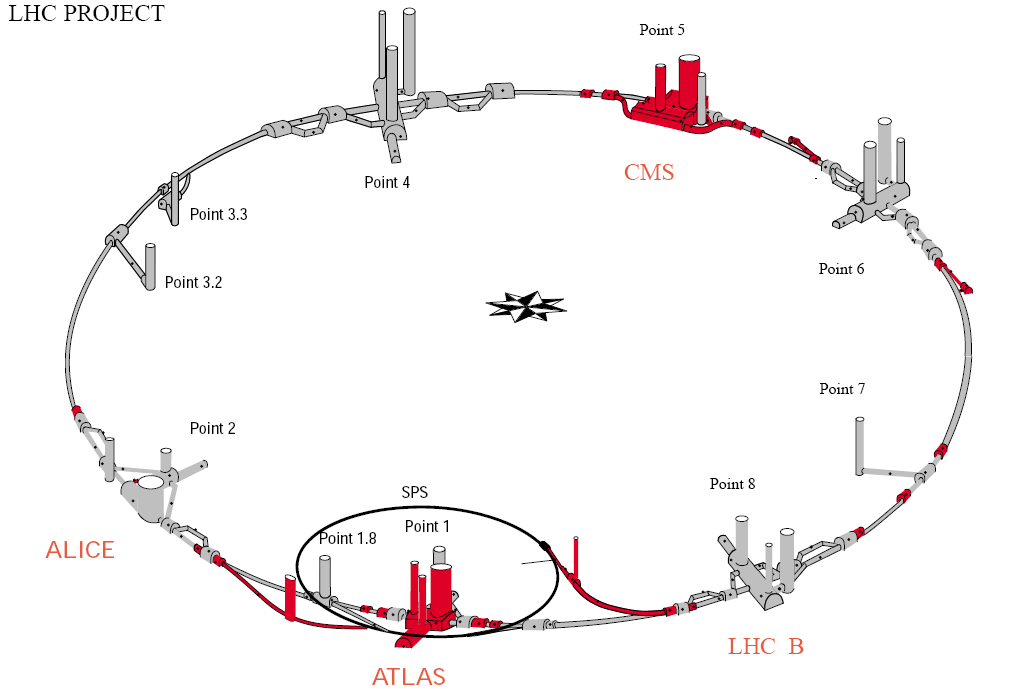
\includegraphics[width=0.8\textwidth]{LHC}
  \caption{An overview of the LHC showing the position of the four main experiments.}
  \label{fig:LHC}
\end{figure}

There are four main detector experiments studying the collisions at the LHC. 
ALICE (A Large Ion Collider Experiment) is designed to study the quark gluon
plasma that will be produced in the heavy ion collisions. 
LHCb (The Large Hadron Collider beauty) experiment is designed to study B-meson
decays to measure CP violation. 
ATLAS (A Toroidal Lhc ApparatuS) and CMS (Compact Muon Solenoid) are general
purpose detectors that are designed 
to search for a wide range of new physics.\cite{lhc}

\section{CMS detector}

\begin{figure}[htb!]
  \centering
  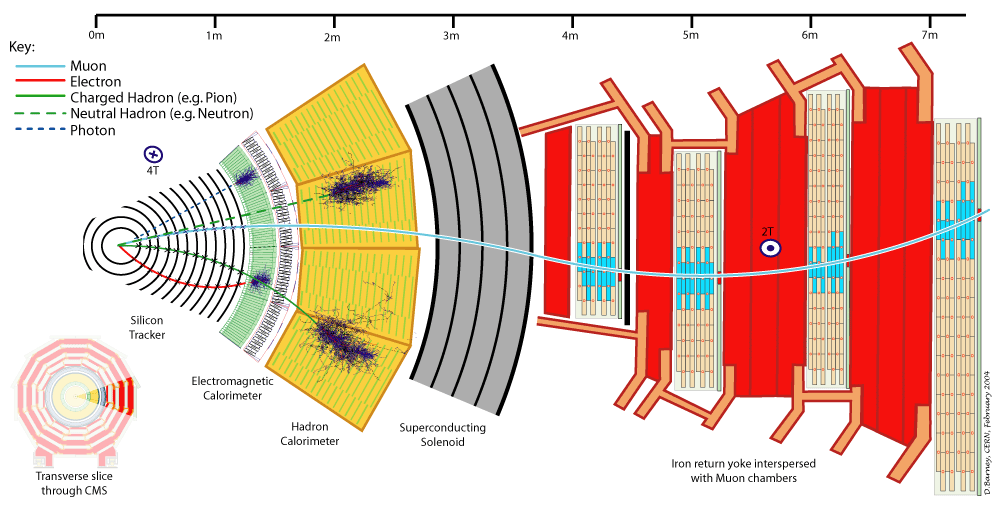
\includegraphics[width=0.8\textwidth]{CMS_Slice}
  \caption{A slice of the CMS detector in the transverse plane showing a
typical response to several different particles. 
From \cite{cmsSlice}.}
  \label{fig:CMS_Slice}
\end{figure}

\begin{figure}[htb!]
  \centering
  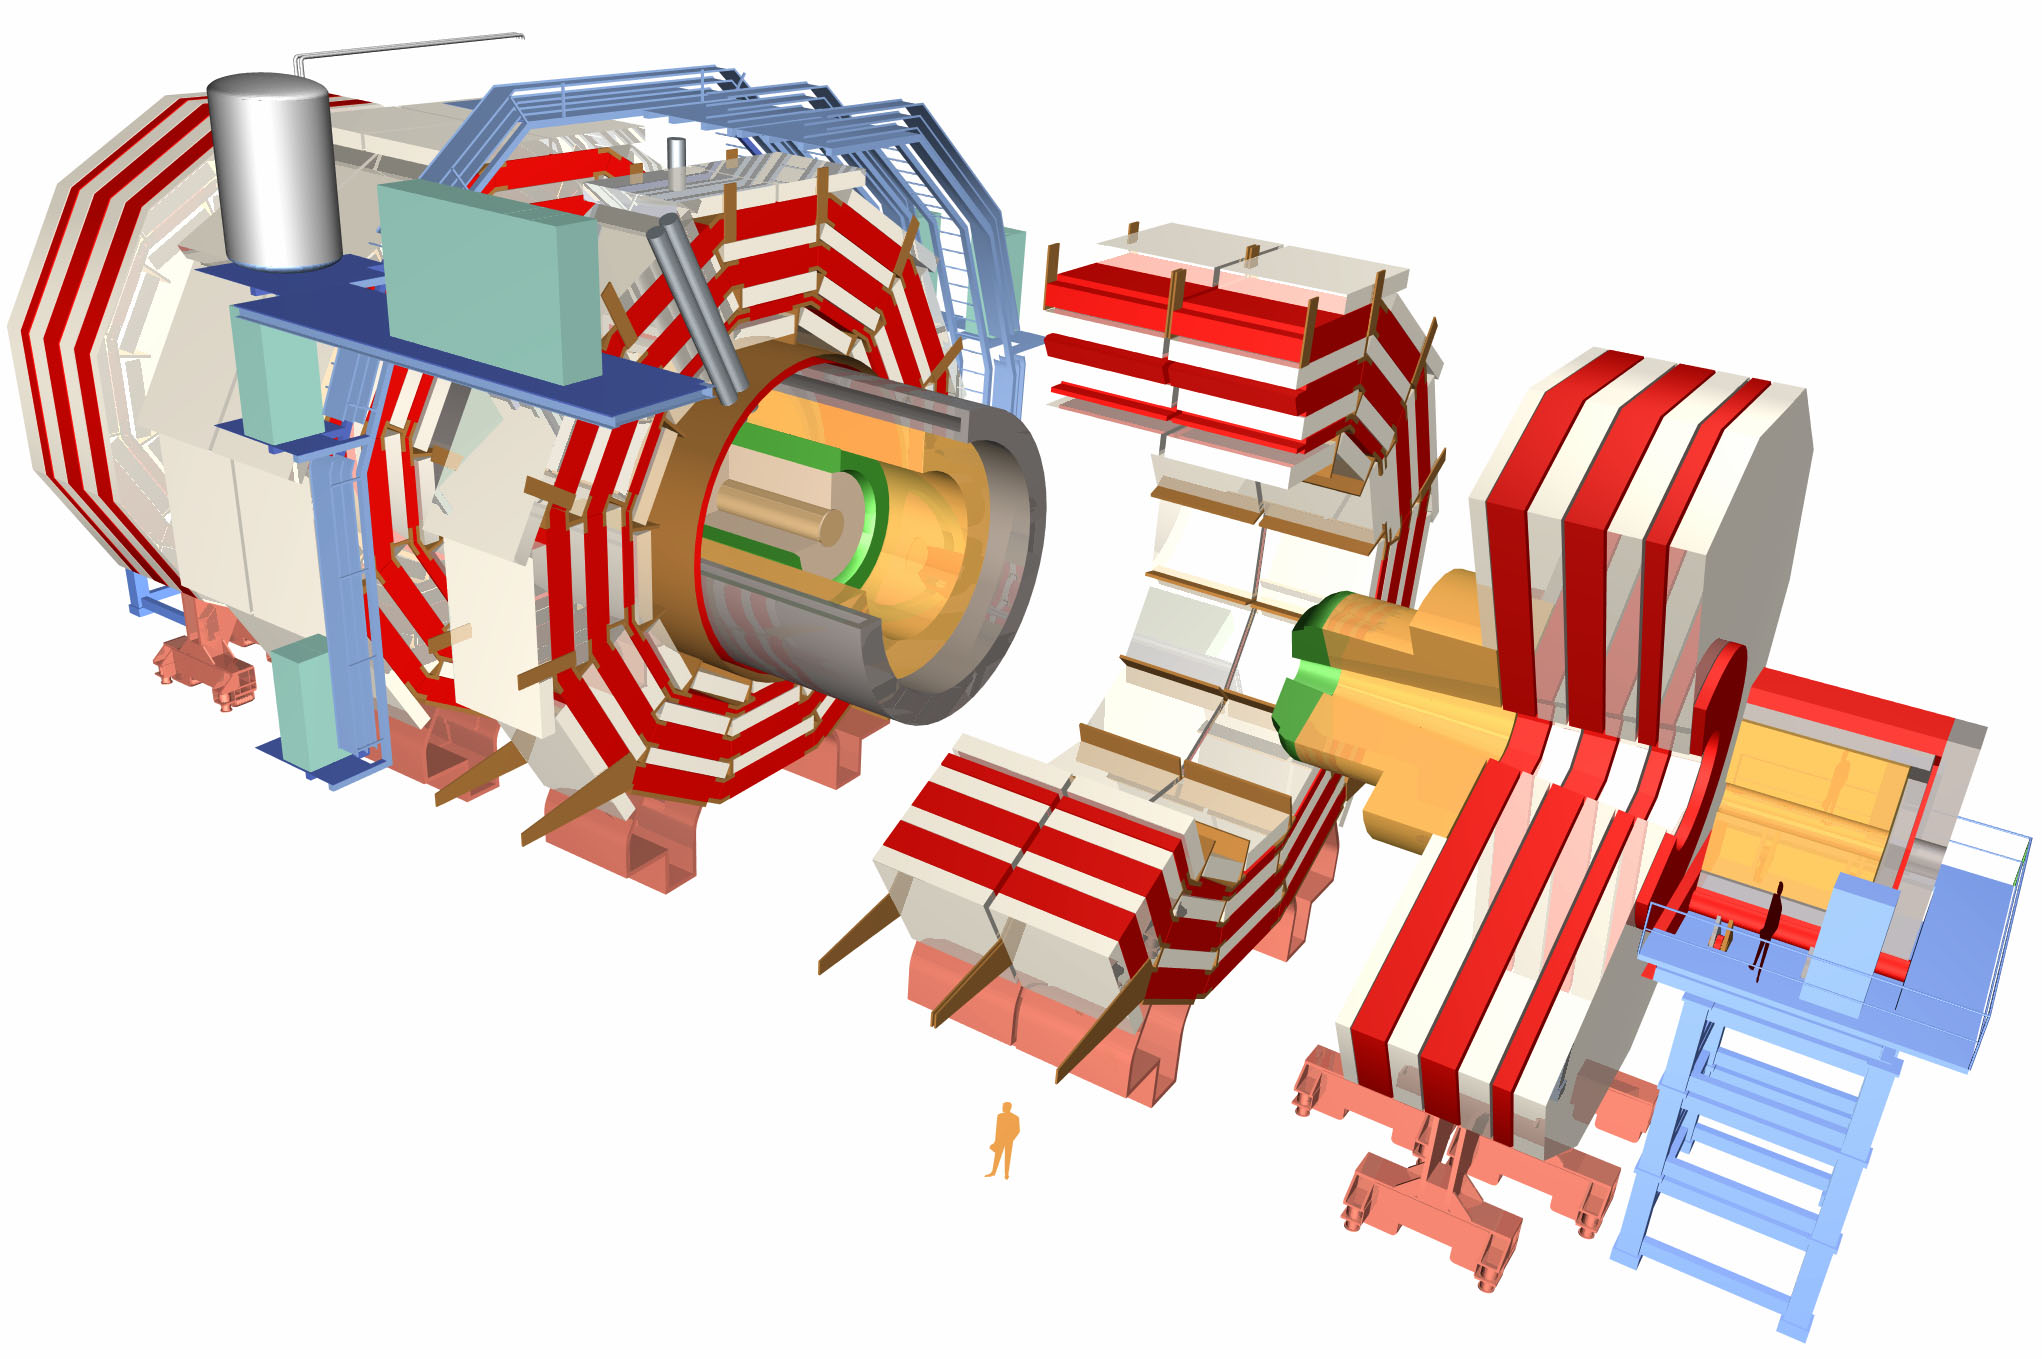
\includegraphics[width=0.8\textwidth]{CMSnc}
  \caption{Diagram of the CMS detector. From \cite{cms}}
  \label{fig:CMSnc}
\end{figure}

CMS (Compact Muon Solenoid)\cite{cms} is one of the two general purpose
detectors designed to study LHC collisions. 
A diagram of a transverse slice of the detector is shown in figure
\ref{fig:CMS_Slice}. 
A large superconducting solenoid that produces a magnetic field of
\unit{4}{\tesla} provides the basis for the design of the CMS detector. 


\subsection{Magnet}
The superconducting magnet in CMS is designed to produce a \unit{4}{\tesla}
field in a bore of 
\unit{6}{\meter} diameter and \unit{12.5}{\meter} length.
While operating at full current the magnet stores \unit{2.6}{\giga\joule} of
energy.
A large magnetic field is needed to give CMS a large bending power and the
ability to precisely measure the momentum of high-energy charged particles.
The solenoid bore is large enough that the tracking detectors and the
calorimetry can fit inside it.\cite{cms}

\subsection{Tracking}
The inner tracker is designed to accurately and efficiently measure the
trajectories of charged particles produced 
in collisions at the centre of CMS.
The tracker is also required to be able to reconstruct secondary vertices
caused by the decay of a long lived particle.
At the design luminosity of the LHC it is expected that every 25 ns an average
of 1000 particles will traverse the 
inner detector therefore it is required that the inner tracker has a high
granularity and a fast response while 
resilient to radiation damage. 
The tracker is therefore based on silicon detectors.
The inner most part of the CMS tracker used silicon pixel detectors arranged in
the barrel section in three layers, 
with the closest layer being at a radius of \unit{44}{\milli\meter}, and in
each endcap region two disks.
The tracking detector also utilises 10 layers of silicon micro-strip detectors
in the barrel region, 
with the outermost layer at \unit{1.1}{\meter} radius, and in 3 plus 9 rings in
the endcap section.
The total active area of silicon in the CMS tracker is over
\unit{200}{\meter\squared}.\cite{cms}

\subsection{Electromagnetic Calorimetry}
The electromagnetic calorimeter (ECAL) is designed to measure the energy of
particles with a high resolution and granularity.
The ECAL utilises 61200 individual lead tungstate ($PbWO_{4}$) scintillation
crystals in the barrel part and 7324 
in each of the two endcap parts. 
Lead tungstate crystals are ideally suited for this since the scintillation
decay time is similar to the LHC 
bunch crossing time with \unit{80}{\%} of light being produced within
\unit{25}{\nano\second} and the short 
radiation length and high density gives a high stopping power which allows the
ECAL to be compact.
A disadvantage to using lead tungstate is that the light output of the crystals
is relatively low and changes 
with temperature so that at \unit{18}{\celsius} 4.5 photoelectrons are
collected per \MeV.
Silicon avalanche photodiodes (APDs) are used to detect the scintillation light
in the barrel and vacuum 
phototriodes (VPTs) are used in the endcap parts.
Installed in front of the endcap ECAL is a preshower system which allows for
the rejection of \Ppizero .\cite{cms}

\begin{figure}[htb!]
  \centering
  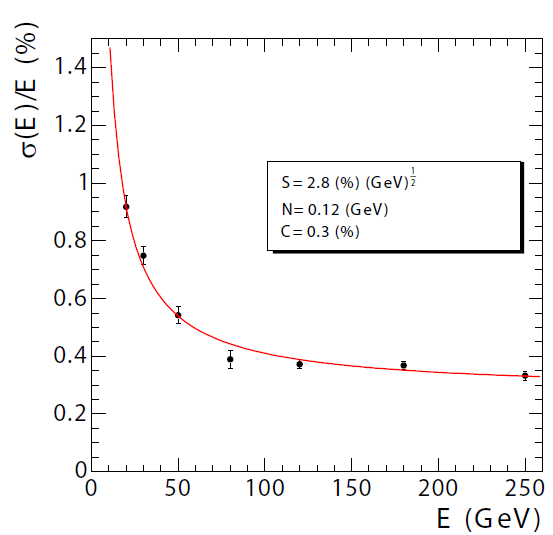
\includegraphics[width=0.6\textwidth]{ECAL}
  \caption{Energy resolution $\frac{\sigma}{E}$ of ECAL as a function of
  \label{fig:ECAL}
electron energy $E$. From \cite{cms}.}
\end{figure}

The ECAL energy resolution is shown in figure \ref{fig:ECAL} for test beam
electrons at several energies ($E$) and is fitted with the function
\begin{equation}
\left(\frac{\sigma}{E}\right)^{2} = \left(\frac{S}{\sqrt{E}}\right)^{2} +
\left(\frac{N}{E}\right)^{2} + C^{2}
\end{equation}
where S is the stochastic, N is the noise and C is the constant terms. The
stochastic term is due to the statistical fluctuations in the particles
produced in the electromagnetic shower. The noise term is due to electronic
noise and pile-up and is independent of energy. The constant term is due to
errors that are independant of energy, such as non-uniform signal generation
and calibration errors.\cite{cms}

% \subsubsection{ECAL Spikes!?}


% \subsubsection{ECAL Endcap Misalignment!?}
% It was found in early data taking that the ECAL endcaps are misaligned with
% respect to the tracker. This causes problems when reconstructing electrons
% since the difference between the track position and ECAL energy deposit is a
% variable that is cut on in the electron candidate selection. As a quick fix
% to this problem, an 

\subsection{Hadronic Calorimetry}
The Hadronic Calorimeter (HCAL) is important in measuring the energy of of
hadron jets and the missing transverse energy (\met) which are important
signatures in many New Physics searches.
A brass/scintillator sampling hadronic calorimeter (HCAL) surrounds the ECAL in
the barrel ($|\eta| < 1.4$) and endcap region ($|\eta| < 3$). 
The scintillation light is channelled by wavelength shifting fibres, that are
embedded in the scintillation tiles, to hybrid photodiodes that can operate in
the high magnetic field. \cite{cms}

In the forward region $|\eta| > 3$ energy measurements are made with an
iron/quartz-fibre forward hadronic calorimeter where the Cherenkov light is
detected by photodetectors.\cite{cms}

In the barrel region ($|\eta| < 1.4$) the HCAL is limited in size since it must
fit in the gap between the the ECAL and tracker within its radius (which extend
from near the beam spot to $R = \unit{1.77}{\meter}$) and the solenoid magnet
outside of it (which starts at $R = \unit{2.95}{\meter}$).
Therefore the total amount of material to absorb the hadronic shower is
limited; to overcome this an outer hadronic calorimeter is placed outside the
solenoid to complement the HCAL barrel.\cite{cms}

\begin{figure}[htb!]
  \centering
  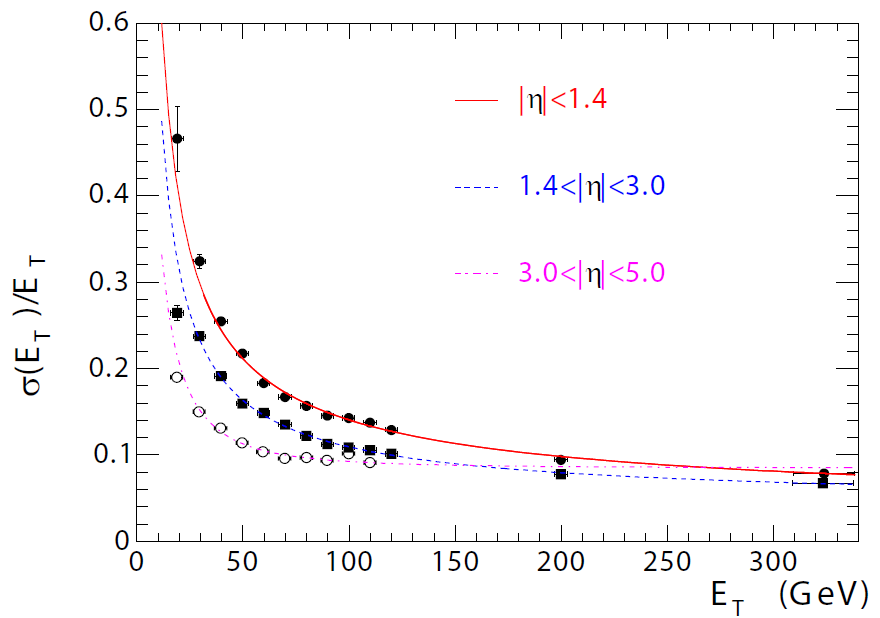
\includegraphics[width=0.8\textwidth]{HCAL}
  \caption{Energy resolution $\frac{\sigma}{E}$ of HCAL as a function of jet
  \label{fig:HCAL}
transverse energy for barrel jets ($|\eta| < 1.4$), endcap jets ($1.4<|\eta| <
3$) and forward jets $3<|\eta| < 5$). From \cite{cms}.}
\end{figure}


\subsection{Muon System}
The muon system lies outside of the CMS solenoid and the outer HCAL detectors,
it is designed to have three functions; to identify muons, measure the momentum
of muons and trigger on muons; to perform these functions the muon system
consists of several different types of detectors. \cite{cms}

In the barrel region ($|\eta| < 1.2$) aluminium drift tubes (DT) are used
arranged in four stations interspersed along the layers of the flux return
plates. 
Each station contains 12 layers, eight to measure the coordinate in the
$r-\phi$ plane and four to measure the $z$ direction (except the fourth station
which only measures the $r-\phi$ plane). 

In the endcaps ($0.9<|\eta|<2.4$) cathode strip chambers (CSC) are used. The
CSCs are arranged in to four stations in each endcap arranged so they are
perpendicular to the beam line, and are placed between the flux return plates.
The cathode strips of each chamber run radially away from the beam line where
as the anode wires run perpendicular to the strips; both are read out which
gives information on both the $r-\phi$ plane (from the cathode) and the $\eta$
direction (from the anode). \cite{cms}

In addition to DT chambers and CSCs a complimentary trigger system is also used
consisting of resistive plate chambers (RPC) in the endcap and barrel regions.
The RPCs are able to provide a fast and independent trigger over a large range
($|\eta| < 1.6$). In the barrel region, 6 layers of RPCs are used, 2 in each of
the first 2 muon stations and 1 in each of the last 2 stations. In the endcap a
layer of RPCs in each of the first 3 stations.

An optical alignment system, that uses lasers and LEDs, measures the positions
of each muon station with respect to each other and the CMS inner tracker to
ensure an accurate and high resolution measurement of the muon
momentum.\cite{cms}

The performance of the muon system and inner tracker is shown in figure
\ref{fig:MS}.

\begin{figure}[htb!]
  \centering
  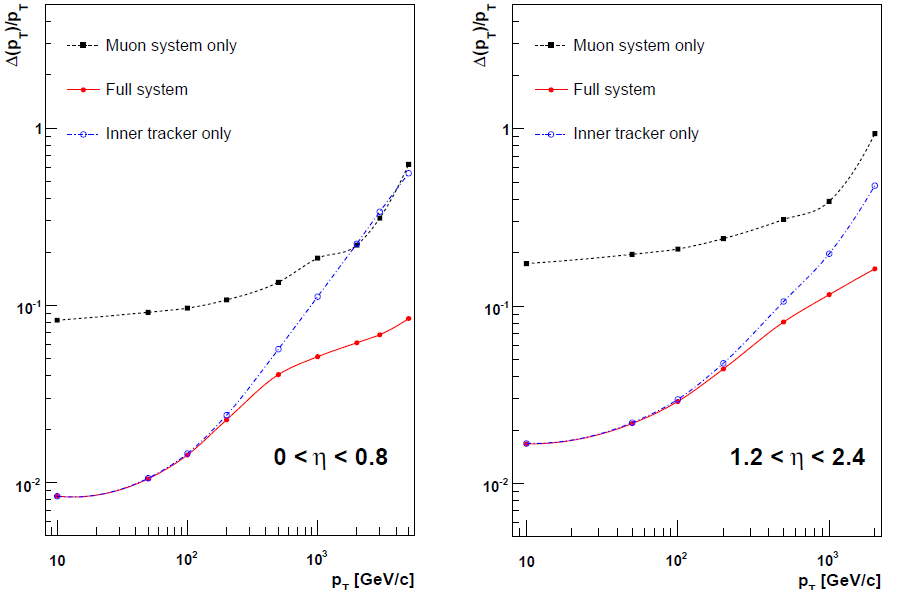
\includegraphics[width=0.8\textwidth]{MS}
  \caption{Muon transverse momentum resolution as a function of the
  \label{fig:MS}
transverse-momentum using only the muon system, only the tracker and both, for
left, barrel muons ($|\eta| < 0.8$) and right, endcap muons ($1.2<|\eta| <
2.4$). From \cite{cms}.}
\end{figure}


\subsection{Trigger and Data Acquisition}
The Data Acquisition and CMS trigger are designed to analyse information from
the detector at the LHC bunch crossing frequency of
\unit{40}{\mega\hertz}\cite{lhc}.
An overview of the DAQ and trigger is shown in figure \ref{fig:CMSDAQ}.

\begin{figure}[htb!]
  \centering
  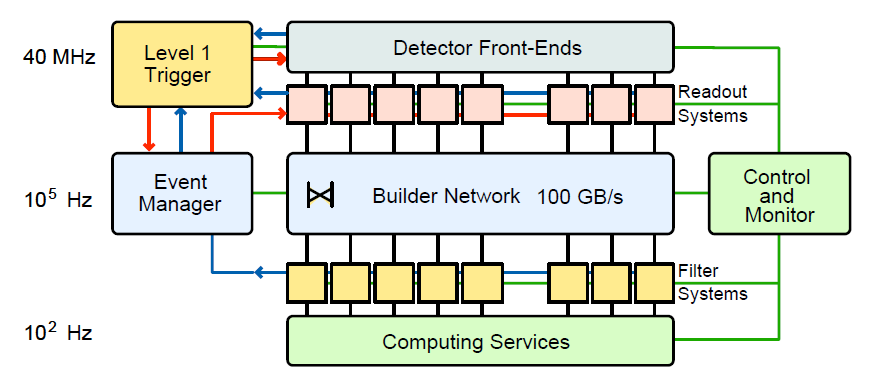
\includegraphics[width=0.6\textwidth]{CMSDAQ}
  \caption{Overview of the architecture of the CMS DAQ and trigger. From
  \label{fig:CMSDAQ}
\cite{cms}.}
\end{figure}

The high bunch crossing frequency of the LHC means that CMS observes and event
every \unit{25}{\nano\second}, however only a small fraction of those event
will be of interest and the vast majority of events will contain only inelastic
collisions.
It is the job of the trigger to drastically reduce this rate while keeping as
many interesting events as possible.
The trigger is separated in to two parts the Level-1 (L1) trigger and the High
Level Trigger (HLT).\cite{cms}

The Level-1 trigger is designed to reduce the event rate from the bunch
crossing frequency of \unit{40}{\mega\hertz} to a maximum output rate of
\unit{100}{\kilo\hertz}.
This is achieved with custom-designed fast programmable electronics that takes
as input coarsely segmented data from the calorimeters and muon systems and
places the high resolution data in pipelined memories.

The high-level trigger is a software system which runs on a server farm with
over one thousand commercial multi-core processors with access to the complete
event data allowing it to make more complex calculations. After the L1 trigger
and HLT the rate is reduced by a factor of $1 \eexp 6$ and is output to mass
storage.\cite{cms}

